\documentclass[a4paper,fleqn,usenatbib]{mnras}

%=========================================================================
\usepackage{amsmath} 
\usepackage{amssymb} 
\usepackage{multirow}

\usepackage{graphicx}
\usepackage{grffile}
\usepackage[dvips]{epsfig}
\usepackage{epsfig}  
\usepackage{color}
\usepackage{caption}
\usepackage{hyperref}
\usepackage{bm}
%Non reposionated tables




%=========================================================================
%		INTERNAL MACROS
%=========================================================================
\def\be{\begin{equation}}
\def\ee{\end{equation}}
\def\ba{\begin{eqnarray}}
\def\ea{\end{eqnarray}}

% To highlight comments 
\definecolor{red}{rgb}{1,0.0,0.0}
\newcommand{\red}{\color{red}}
\definecolor{darkgreen}{rgb}{0.0,0.5,0.0}
\newcommand{\SRK}[1]{\textcolor{darkgreen}{\bf SRK: \textit{#1}}}
\newcommand{\SRKED}[1]{\textcolor{darkgreen}{\bf #1}}
\newcommand{\before}[1]{\textcolor{red}{ #1}}
\newcommand{\after}[1]{\textcolor{darkgreen}{ #1}}
\newcommand{\hs}{{\hspace{1mm}}}  
\newcommand{\tol}{Tololo 1214-277}
\newcommand{\rank}{\texttt{Ranked}}
\newcommand{\boot}{\texttt{Bootstrapped}}
\newcommand{\rand}{\texttt{Random}}
\newcommand{\HI}{{\text{H\MakeUppercase{\romannumeral 1}}} }
\newcommand{\HII}{{\text{H\MakeUppercase{\romannumeral 2}}} }
\newcommand{\lya}{\ifmmode{{\rm Ly}\alpha}\else Ly$\alpha$\ \fi}
\newcommand{\cm}{\ifmmode{{\rm cm}}\else cm\fi}
\newcommand{\ccm}{\,\mathrm{cm}^{-3}}
\newcommand{\ergps}{\,{\rm erg}\,{\rm s}\ifmmode{}^{-1}\else ${}^{-1}$\fi}
\newcommand{\Mpch}{\,{\rm Mpc}\,\ifmmode h^{-1}\else $h^{-1}$\fi}
\newcommand{\dd}{\mathrm{d}}
\newcommand{\vek}[1]{\bm{#1}}
\newcommand{\hb}{H$\beta$}
\newcommand{\ha}{H$\alpha$}
\newcommand{\oiii}{[OIII]}
\newcommand{\oii}{[OII]}
\newcommand{\nii}{[NII]}
\newcommand{\esca}{erg cm$^{-2}$ s$^{-1}$ \AA$^{-1}$}
\newcommand{\esc}{erg cm$^{-2}$ s$^{-1}$}
\newcommand{\es}{erg s$^{-1}$}
\newcommand{\esa}{erg s$^{-1}$}
\newcommand{\kms}{\ifmmode\mathrm{km\ s}^{-1}\else km s$^{-1}$\fi}
\newcommand{\hMsun}{{\ifmmode{h^{-1}{\rm{M_{\odot}}}}\else{$h^{-1}{\rm{M_{\odot}}}$}\fi}}
\newcommand{\Msun}{{\ifmmode{{\rm{M_{\odot}}}}\else{${\rm{M_{\odot}}}$}\fi}}

\newcommand{\jefr}[1]{\textcolor{darkgreen}{\bf JEFR: \textit{#1}}}

\begin{document}

%=========================================================================
%		FRONT MATTER
%=========================================================================
\title[LG as an outlier]{We are not the 99 percent: quantifying
  bright satellite distributions in the Local Group}
\author[J.E. Forero-Romero \& V. Arias]
{Jaime E. Forero-Romero $^{1}$ \thanks{je.forero@uniandes.edu.co},
Ver\'onica Arias$^1$\\
%%
$^1$ Departamento de F\'isica, Universidad de los Andes, Cra. 1
  No. 18A-10 Edificio Ip, CP 111711, Bogot\'a, Colombia \\
}

\maketitle

\begin{abstract}
In this paper we quantify the joint spatial distribution of the
brightest satellites around the Milky Way (MW) and M31, the dominant
galaxies in the Local Group (LG).
We use the Illustris-1 and ELVIS simulations to quantify the
expected deviations from statistically spherical satellite
distributions in the Lambda Cold Dark Matter paradigm. 
We estimate that only $0.05\%$ to $0.25\%$ of the pairs with isolation
and dynamical characteristics similar to the LG are expected to have
satellite distributions with the same degree of deviation from
sphericity.
This makes the LG a $3\sigma$ outlier, with all the weight lying on
the extremly planar MW satellite distribution.
\end{abstract}

\begin{keywords}Galaxies: halos --- Galaxies: high-redshift --- Galaxies: statistics
--- Dark Matter --- Methods: numerical 
\end{keywords}

\section{Introduction}

 
It has been shown that LG pair separation vector is aligned along the
filaments in  which they are typically embeded
\cite{2015ApJ...799...45F}, the LG pairs found in pancake-like DM
matter arrangements are aligned with the plane itself. 
Characterizing the satellite alignments with $\mu$ thus provide
information about how satellites are distributed with respect to the
cosmic web. 

In Section we list the sources of the observational and
simulated data to be used throughout the paper.
Next, in Section we describe the methods we use to quantify and
characterize the satellite distributions.
In section we present our results. 
In the discussion section we quantify the correlations between the main
plane properties as described by the simulations.
We use this results to quantify the degree of atipicality of the LG
and estimate the volume that has to probed in simulations in order to
find a pair with a satellite distribution as atipical as the LG. 
Finally, we summarize our conclusions in Section .

\label{Data Samples}

\subsection{Observational Data}
\label{sec:obs}



\subsection{Data from the ELVIS project}
\label{sim:ELVIS}

\subsection{Data from the Illustris project}
\label{sec:illustris}

We use publicly available data from the Illustris Project 
\citep{2014MNRAS.444.1518V}. 
This suite of cosmological simulations, performed using the quasi-Lagrangian
code AREPO \citep{2010MNRAS.401..791S}, followed the coupled evolution of dark 
matter and gas and includes parametrizations to account for the effects of
gas cooling, photoionization, star formation, stellar feedback, black
hole and super massive black hole feedback. 
The simulation volume is a cubic box of $75$ \Mpch\ on a side.
The cosmological parameters correspond to a $\Lambda$CDM cosmology
consistent with WMAP-9 measurements \citep{2013ApJS..208...19H}. 

We extract halo and galaxy information from the Illustris-1 simulation
which has the highest resolution in the current release of the
Illustris Project.
Illustris-1 has $1820^3$ dark matter particles and $1820^3$ initial gas
volumen elements. 
This corresponds to a dark matter particle mass of
$6.3\times 10^6$\Msun\ and a minimum mass for the baryonic volume
element of $8.0\times 10^7$\Msun. 
The corresponding spatial resolution is $1.4$ kpc for the dark matter
gravitational softening and $0.7$ kpc for the typical size of the
smallest gas cell size. 

We buid a sample of Isolated Pairs that resemble the conditions
in the LG.
To construct this sample we select first all galaxies with  an stellar mass in the range $1\times10^{10}\Msun
<M_{\star}<1.5 \times 10^{11} \Msun$.
Then we consider the following criteria for all galaxies in that set.


\begin{itemize}
\item For each galaxy $A$ we find its closest galaxy $B$, if galaxy $A$ is also
the closest to halo $B$, the two are considered as a pair. 
\item With $d_{AB}$ the distance between the two galaxies and
  $M_{\star,min}$ the lowest stellar mass in the two galaxies, we
  discard pairs that have any other galaxy $C$ with stellar mass
  $M_{\star}>M_{\star, min}$ closer than $3\times d_{AB}$ from any of
  the pair's members. 
\item The distance $d_{AB}$ is greater than $700$ kpc.
\item The relative radial velocity between the two galaxies, including
  the Hubble flow, is $-120\ \kms <v_{AB,r}<0\ \kms$. 
\end{itemize}

We find 27 pairs with these conditions. 
We then select the pairs where in both halos there are at least 15
detected subhalos, thus discarding pairs with halos with the lowest
mass.
We end up with a total of 20 pairs that fulfill these criteria,
Appendix A shows the physical  properties (stellar masses, maximum
circular velocities, radial velocities and separation) in those pairs. 


Although Illustris-1 has stellar particles, we do not use their
properties to select the satelite population because the smallest
galaxies are barely resolved in stellar mass at magnitudes of
$M_V=9$. We prefer using the dark matter information as the smallest
sub-halos are sampled with at least $35$ particles. 
We chose the satellite samples by ranking the subhalos in decreasing
order of its maximum circular velocity and select the first $N_p$
halos in the list. 
The results presented here correspond to $11\leq N_p\leq 15$. 

\section{Building, Characterizing and Comparing Satellites Spatial Distributions}
\label{sec:SpatialMeasurements}


\subsection{Building Satellite Samples}

We compare the joint satellite distributions in the MW and M31 at fixed
satellite number, $N_s$.
This means that the magnitude cut corresponding to the faintest
satellite included in the sample is different in each case.
We make this choice for two reasons. 
First, to be sure that there is a non-zero number of satellites in the
simulations to make the computations.  
Second, to rule out the influence of satellite numbers in the
statistics. 

We compute the satellite statistics fo 11 up to 15 satellites.
The lowest bound corresponds to the number of classical Milky Way
satellites.
The upper limit corresponds to the maximum number of satellites that
can be resolved in both halos for most of the isolated pairs in Illustris-1.
In simulations we rank the subhalos by their maximum
circular velocity, in observations we rank the satellites by its $M_V$
magnitude. 

We also use two kinds of satellite distributions. 
The first keeps the positions for the satellites fixed as provided in
the observations/simulations; the second randomizes the angular positions of
the satellites around the central galaxy while keeping its radial
distance fixed. The randomization process is done 1000 times for each
galaxy. 


\subsection{Describing Samples with the Inertia Tensor}
We base all our results on the description provided by the inertia
tensor defined by the satellites's positions.  

\begin{equation}
{\bf{\bar{I}}} = \sum_{k=1}^{N_s}[(\bf{r}_i - \bf{r}_0)^2\cdot \bf{1} -
  (\bf{r}_i-\bf{r}_0)\cdot (\bf{r}_i - \bf{r}_0)^{T}],
\end{equation}
%
where $k$ indexes the set of satellites of interest
$\bf{r}_k$ are the satellites' positions, $\bf{r}_{0}$ is the location
of the central galaxy $\bf{1}$ is the unit matrix,  and  
${\bf r}^T$ is the transposed vector $\bf{r}$. 
We use $\bf{r}_0$ as the position of the central galaxy, and not the
satellites' geometrical center, to allow for a fair comparison once
the angular positions of the satellites are randomized around this
point. 

From this tensor we compute its eigenvalues,
$\lambda_1>\lambda_2>\lambda_3$, and corresponding eigenvectors,
$\hat{I}_1$, $\hat{I}_2$, $\hat{I}_3$.
We define the size of the three ellipsoidal axis as
$a=\sqrt{\lambda_1}$, $b=\sqrt{\lambda_2}$ and $c=\sqrt{\lambda_3}$.
We also define $\hat{n}\equiv \hat{I}_1$ as the vector perpendicular to the
planar satellite distribution. 
We also define the width, $w$, of the planar satellite distribution,
$\sigma_p$ as the standard deviation of all satellite distances to the
plane defined by the vector $\hat{n}$. 
Finally, we characterize the alignment between the satellite plane and the
vector connecting the two dominant galaxies by $\mu=|\hat{r}_{AB}\cdot
\hat{n}|$.

To summarize we characterize the satellite distribution by for
quantities obtained from the inertia tensor: 
\begin{itemize}
\item Plane width, $w$.
\item $c/a$ axis ratio.
\item $b/a$ axis ratio.
\item $\mu$ as a measure of plane alignment.
\end{itemize}


\subsection{Comparing Satellite Samples}


\subsection{Describing joint satellite distributions}


% referencia posiciones satellites
% http://adsabs.harvard.edu/abs/2013MNRAS.435.1928P

\begin{figure*}
\centering
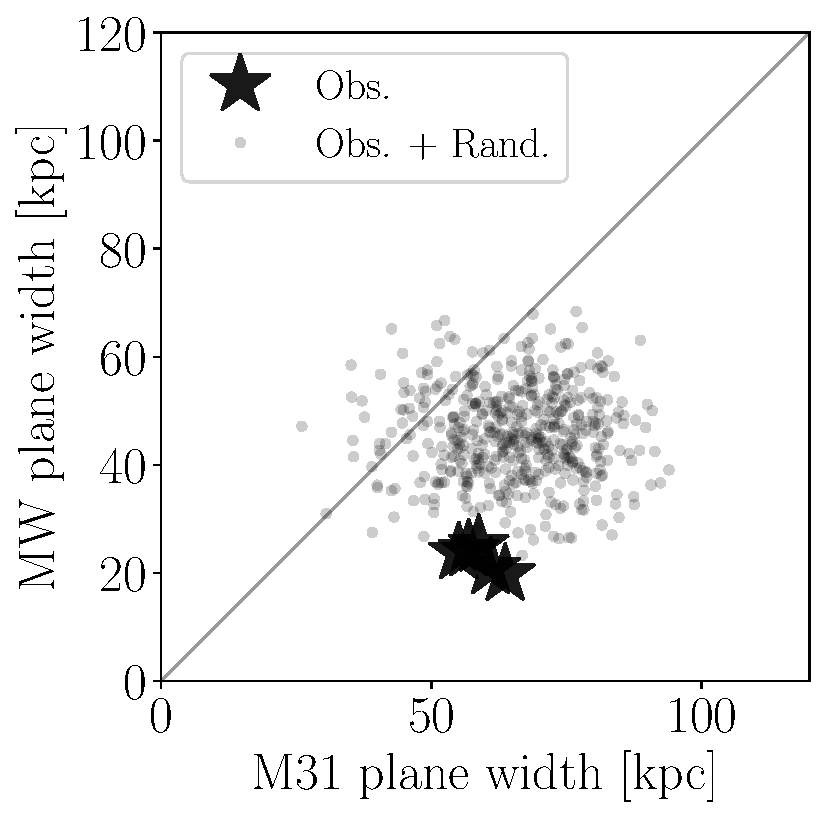
\includegraphics[width=0.32\textwidth]{scatter_random_ranked_width.pdf}
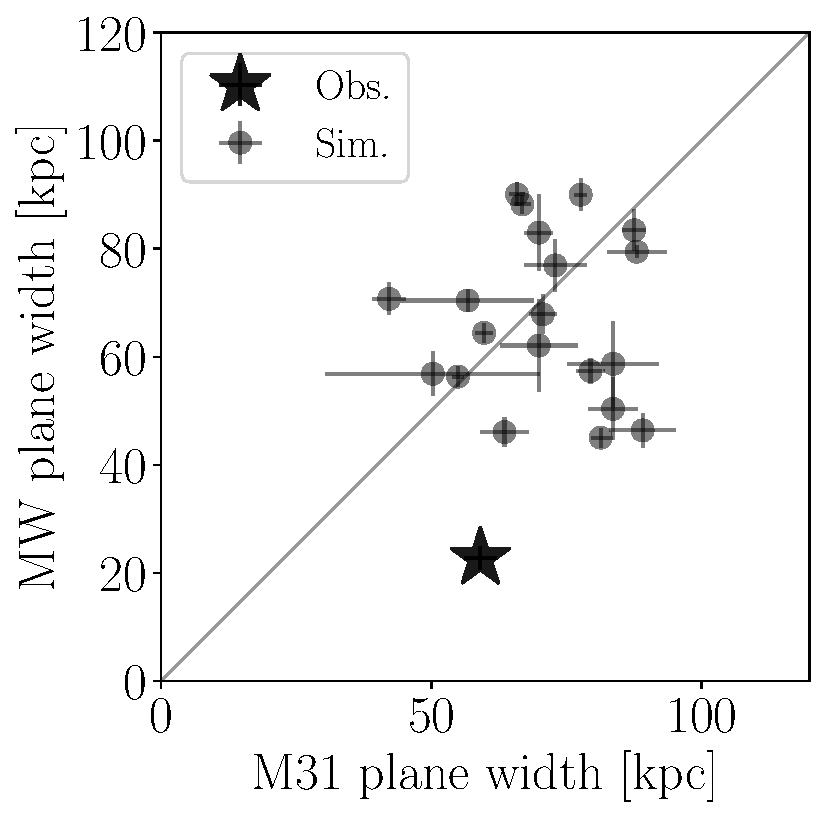
\includegraphics[width=0.32\textwidth]{scatter_ranked_width.pdf}
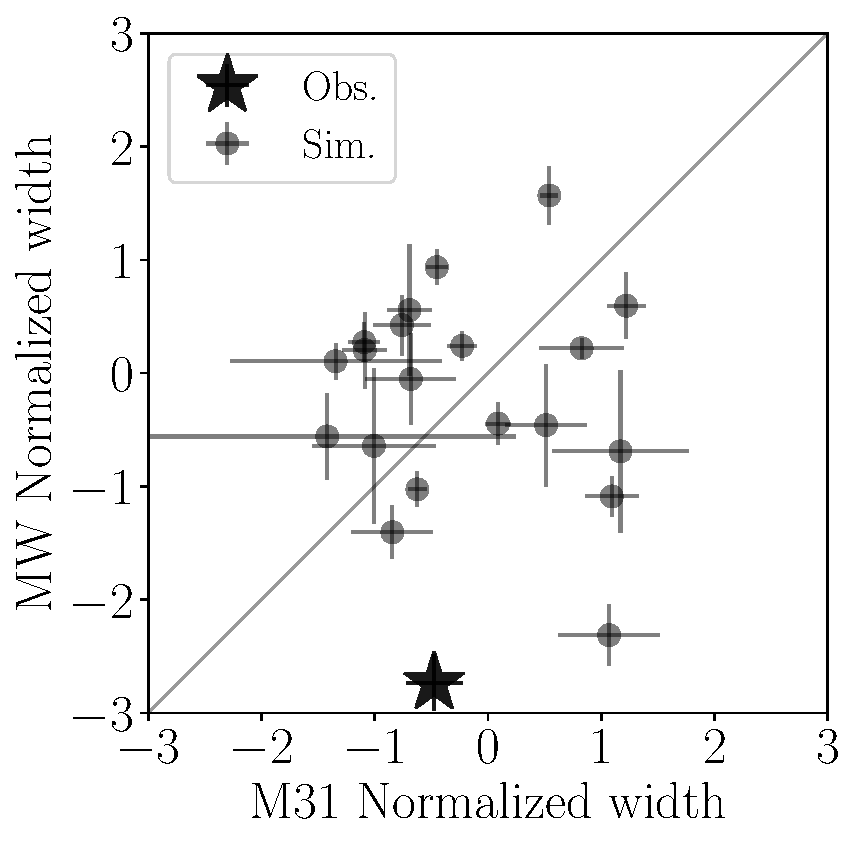
\includegraphics[width=0.32\textwidth]{scatter_norm_ranked_width.pdf}
\caption{Plane width characterization in the Local Group and the
  Isolated Pairs. In all panels the horizontal axis corresponds to the
  M31 or the most massive halo in the pair and the vertical axis to
  the MW or the least massive halo in the pair.
The panel on the left shows the plane width in physical units
comparing the results from observations
(stars) against the result of spherically randomizing the satellite
positions while keeping its radial distance (circles). 
The panel in the middle compares the average from the observations
(star) and the average from each one of the Isolated Pairs (circles
with error bars).
The panel on the right has the same information as the middle panel,
only that this time each point has been normalized (median substracted
and normalized by the standar deviation) to the results of its
randomization. 
The main message of this series of plots is that the MW has a
significantly thiner plane both compared to the result of its own
satellite spherical randomization (left panel) and the expectation from
simulations (middle panel). 
This low value is $2\sigma$ away from what is expected in a spherical
distribution. 
In the M31 their satellites are in agreement with the expectations
both from an spherical distribution and the results form the
simulations. 
A second conclusion is that the spherically averaged plane width
MW (seen in the point cloud in the left panel) is smaller than the
average expectation from simulations, while for M31 the spherical
average is consistent with simulations. 
\label{fig:scatter_width}}
\end{figure*}

\begin{figure*}
\centering
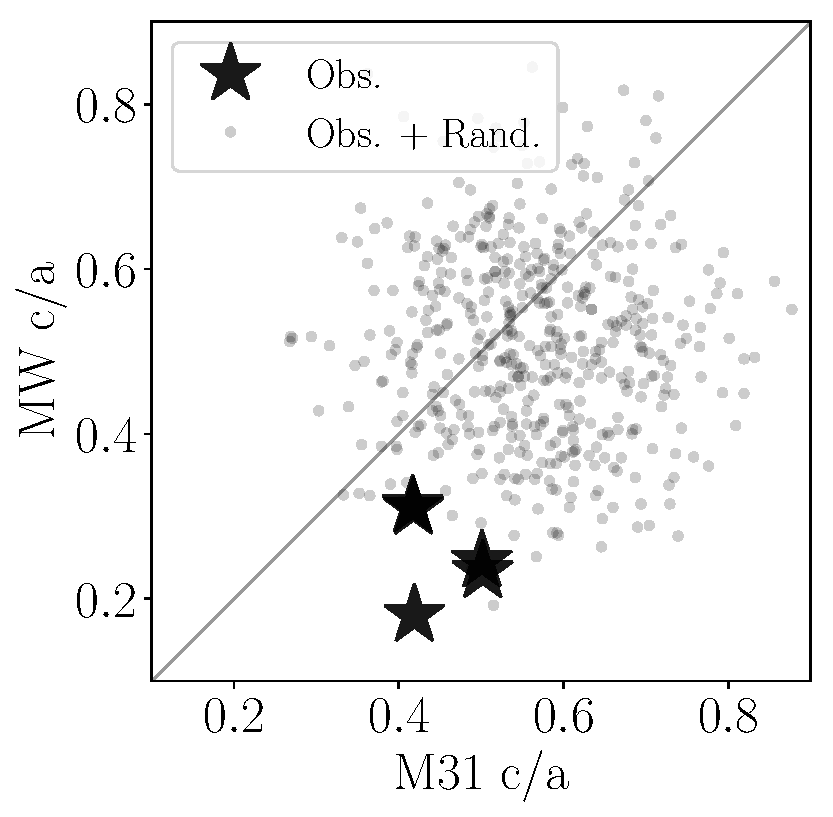
\includegraphics[width=0.32\textwidth]{scatter_random_ranked_ca_ratio.pdf}
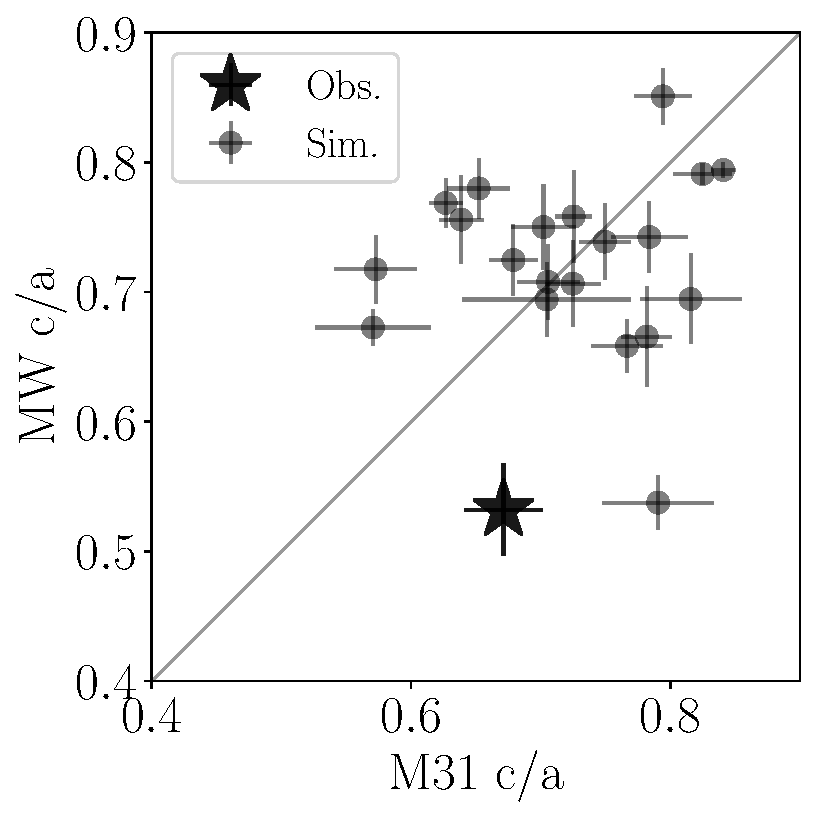
\includegraphics[width=0.32\textwidth]{scatter_ranked_ca_ratio.pdf}
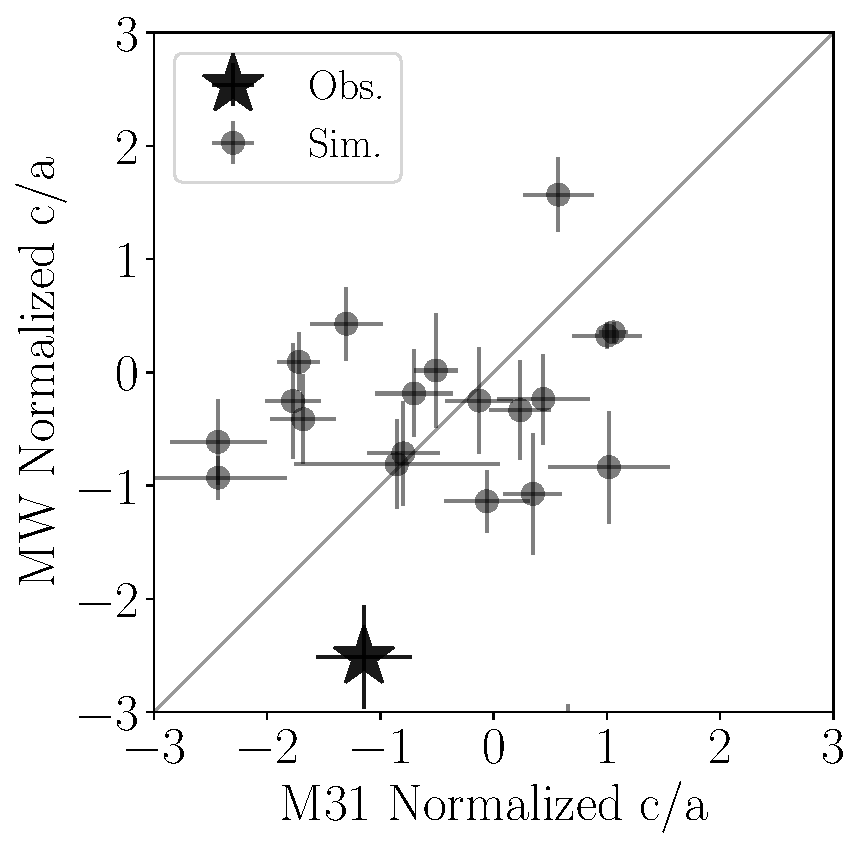
\includegraphics[width=0.32\textwidth]{scatter_norm_ranked_ca_ratio.pdf}
\caption{Same layout as in Figure \ref{fig:scatter_width}. 
This time for the $c/a$ axis ratio. 
The message holds in this case as for the plane width.
The MW is has a significantly low $c/a$ value compared to the
expectation from a spherical distribution and simulations. 
This low value is also $2\sigma$ away from the expactations for an
spherical distribution.
M31 is consistent both with an spherical distribution and the results
from simulations.
However, in this case the axis ratio in the spherically averaged case
is completeley consistent with the expectation from simulations.
\label{fig:scatter_ca_ratio}}
\end{figure*}


\begin{figure*}
\centering
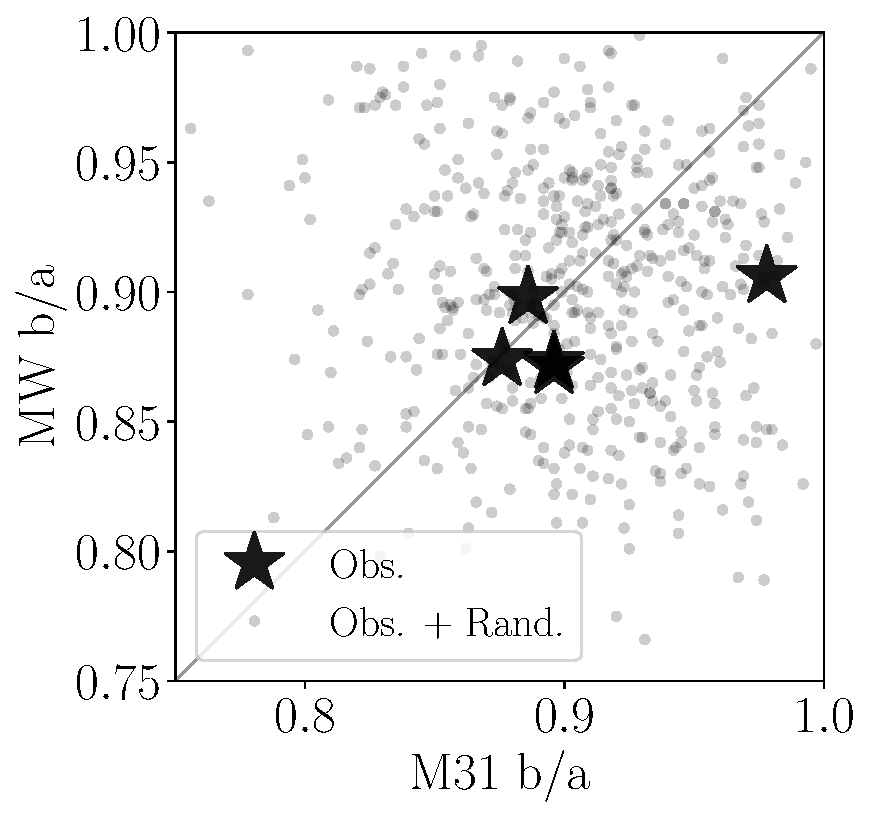
\includegraphics[width=0.32\textwidth]{scatter_random_ranked_ba_ratio.pdf}
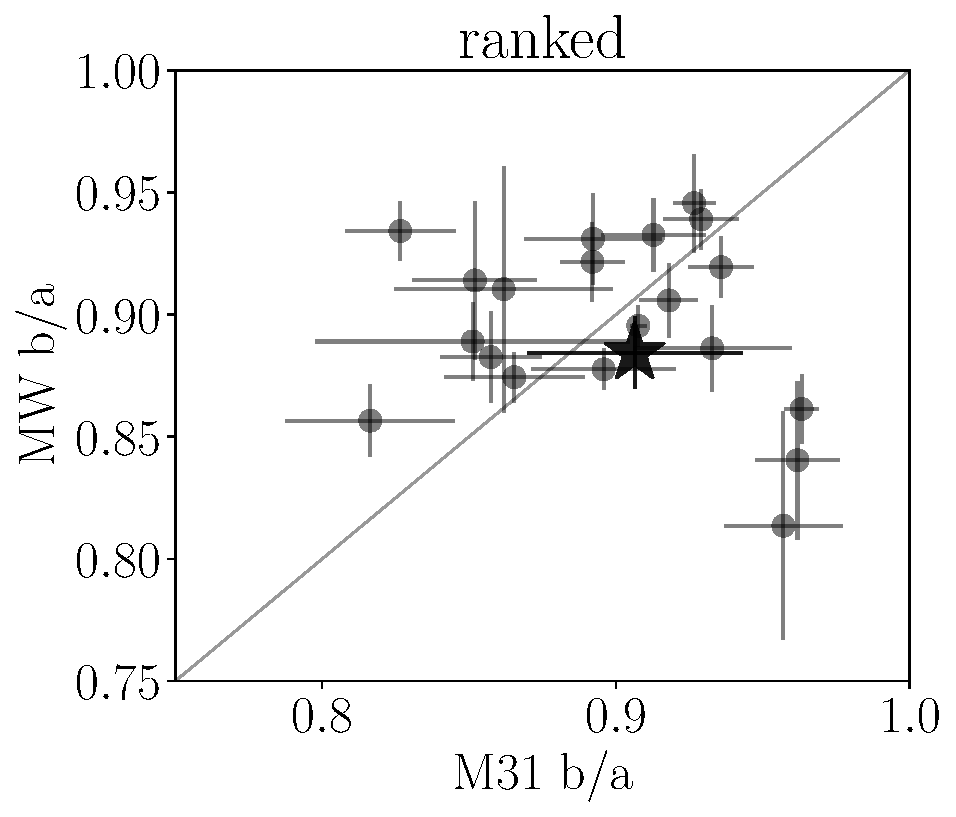
\includegraphics[width=0.32\textwidth]{scatter_ranked_ba_ratio.pdf}
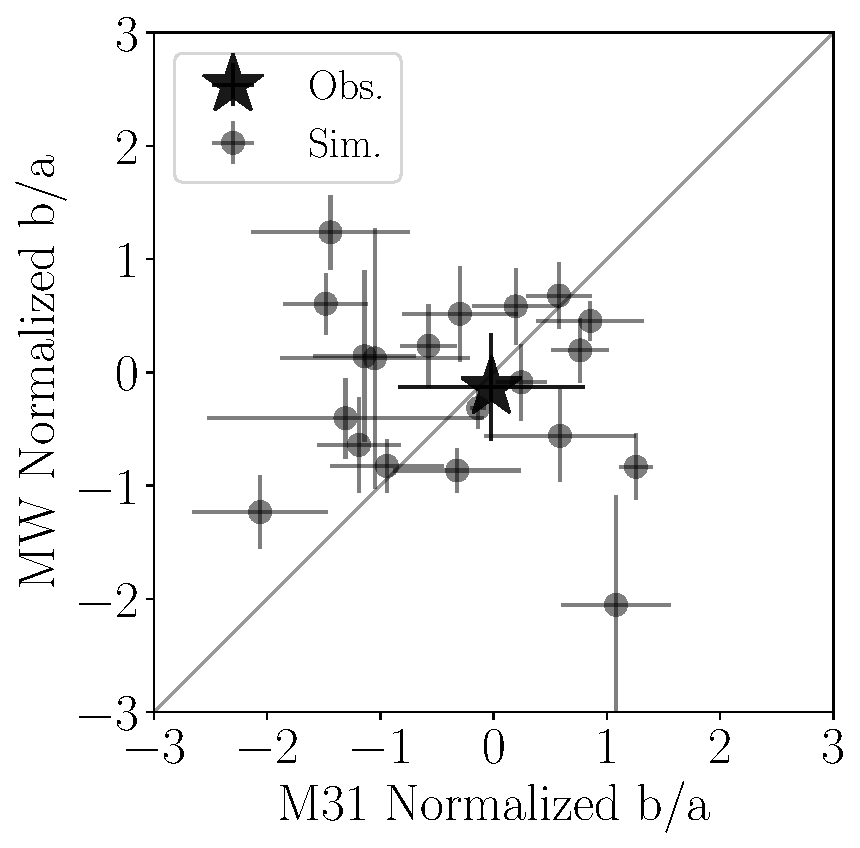
\includegraphics[width=0.32\textwidth]{scatter_norm_ranked_ba_ratio.pdf}
\caption{Same layout as in Figure \ref{fig:scatter_width}. 
This time for the $b/a$ axis ratio. In this case both the MW and M31
are consistent with the results of a spherical distribution and the
simulations. 
\label{fig:scatter_ba_ratio}}
\end{figure*}

\begin{figure*}
\centering
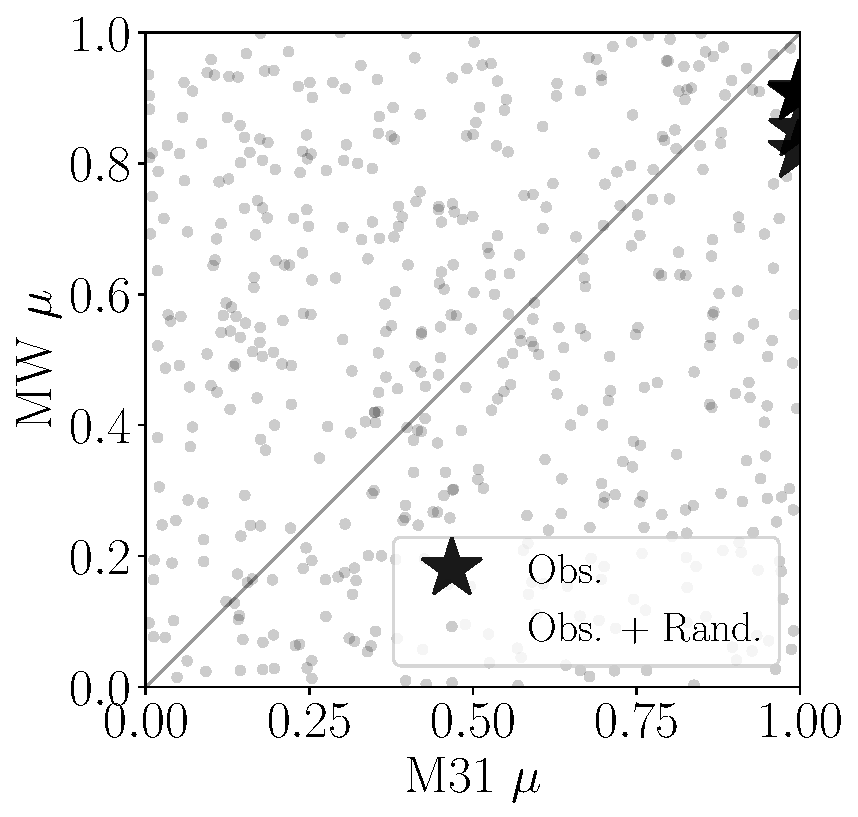
\includegraphics[width=0.32\textwidth]{scatter_random_ranked_mu.pdf}
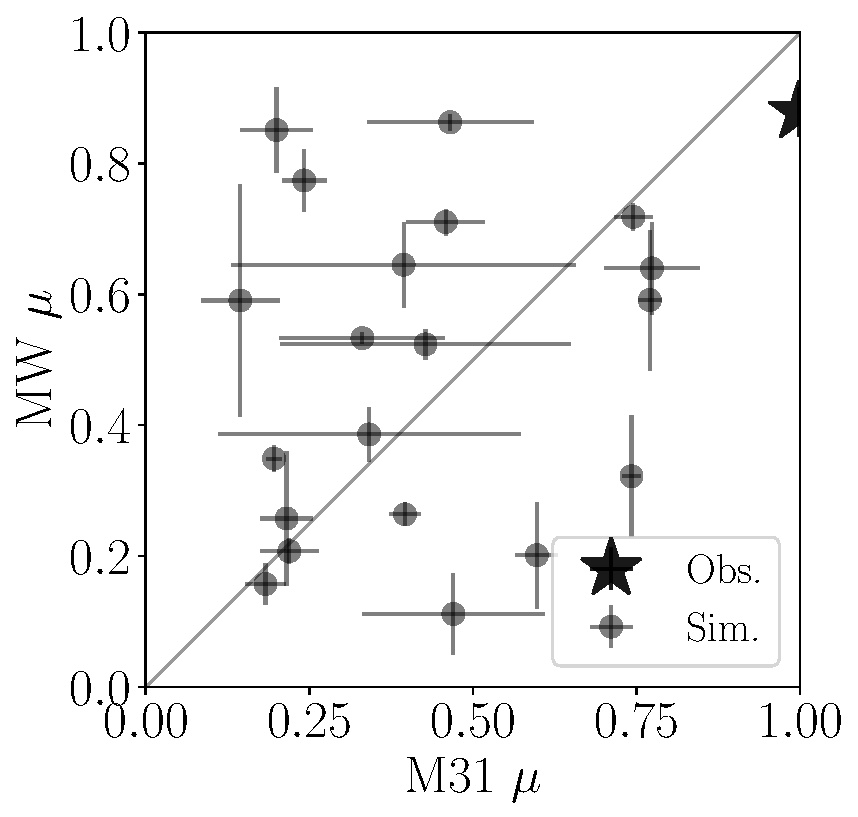
\includegraphics[width=0.32\textwidth]{scatter_ranked_mu.pdf}
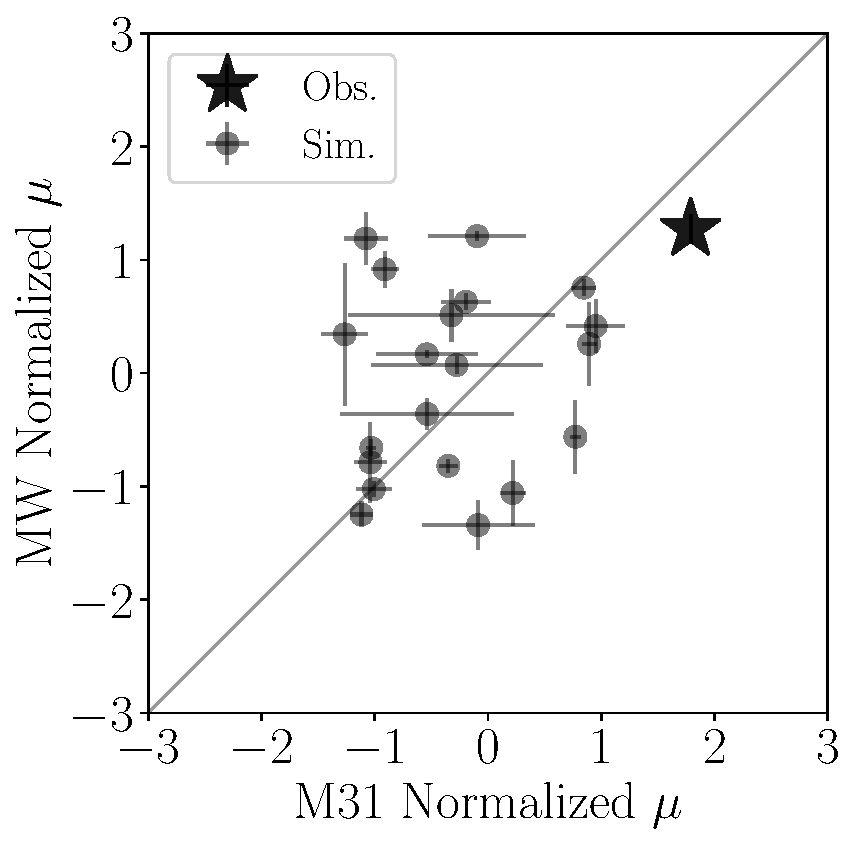
\includegraphics[width=0.32\textwidth]{scatter_norm_ranked_mu.pdf}
\caption{Same layout as in Figure \ref{fig:scatter_width}. 
This time for $\mu$ the absolute value of the dot product between the
vector connecting the main galaxies and the vector perpendicular to
the satellite plane.
In this case both the MW and M31 show a strong alignment.
Apparently the LG is outside the expectations from
simulations and atypical compared to the spherical results. 
However, this is not the case. The $\mu$ distributions in the
randomization and the simulation are consistent with a uniform
distribution.
Under such circumstances $\mu\approx 1$ is as likely as
any other value.
\label{fig:scatter_mu}}
\end{figure*}


\begin{figure*}
\centering
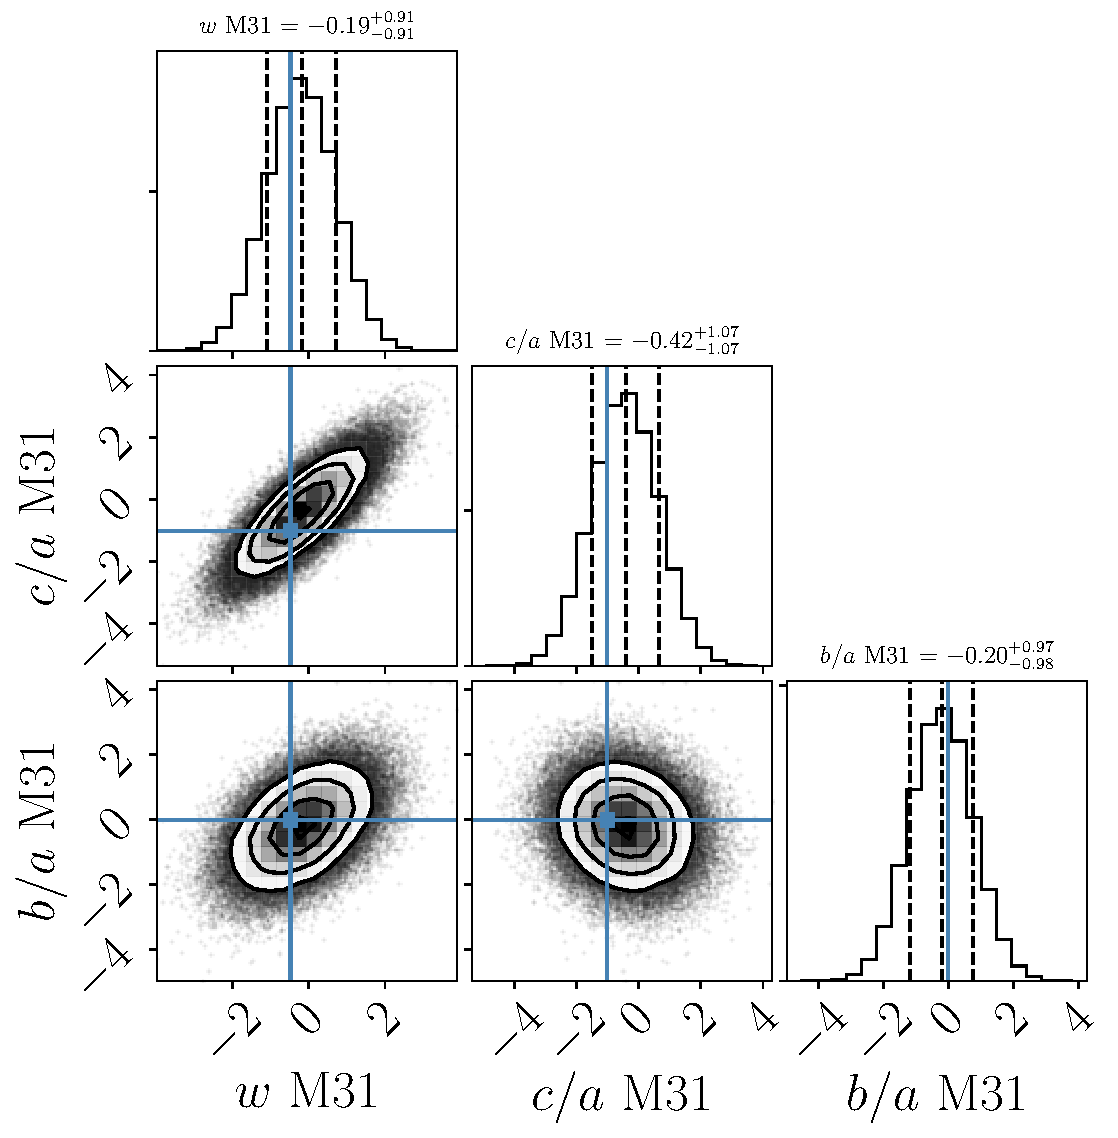
\includegraphics[width=0.45\textwidth]{gaussian_model_illustris_M31.pdf}
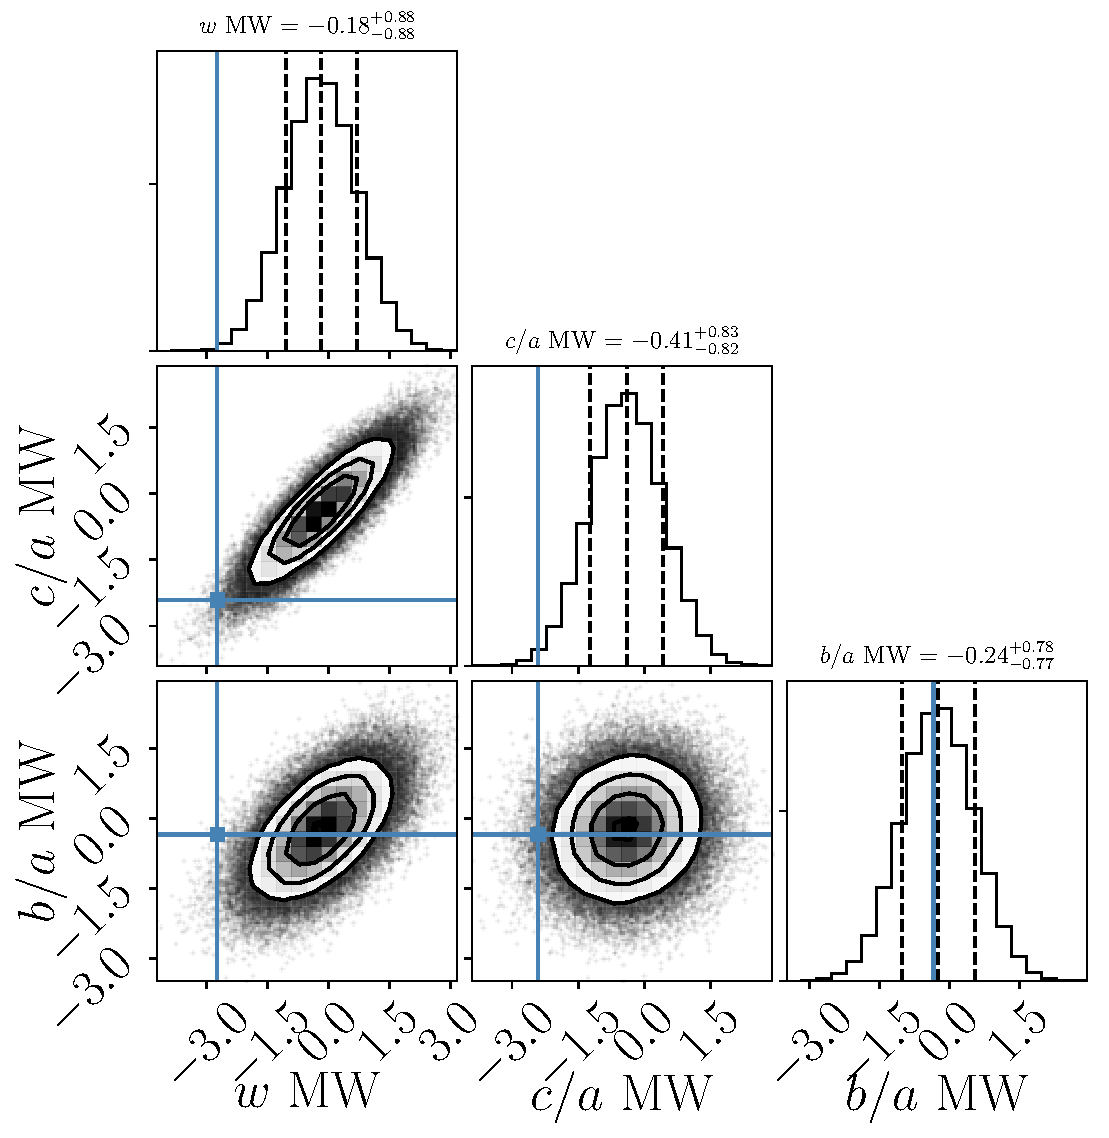
\includegraphics[width=0.45\textwidth]{gaussian_model_illustris_MW.pdf}
\caption{Correlations between the multivariate gaussian model built on
  the normalized values for the plane width $w$, $c/a$ ratio and $b/a$ ratio. 
Left/right panel correspond to M31/MW. 
The contour levels in the 2D histograms correspond to the $1\sigma$,
$2\sigma$ and $3\sigma$ contours in two dimensions. 
The dahsed vertical lines in the histograms along the diagonal
correspond to the $1\sigma$ boundaries in one dimension.
The results for the gaussian model are built from $10^6$ point
realizations in the six-dimensional space spaned by the variables of
interest. 
The correlation matrix and the mean values are computed from the
results in the Illustris-1 simulation.
The cross indicates the LG values.
This plot clearly shows how the M31 results are well within the
expectations from simulations while MW has an unusual low value for
the plane width and the $c/a$ axis ratio.
Equivalent results from the ELVIS data are presented in Figure
\ref{fig:correlations_elvis}.
\label{fig:correlations_illustris}}
\end{figure*}


\begin{figure}
\centering
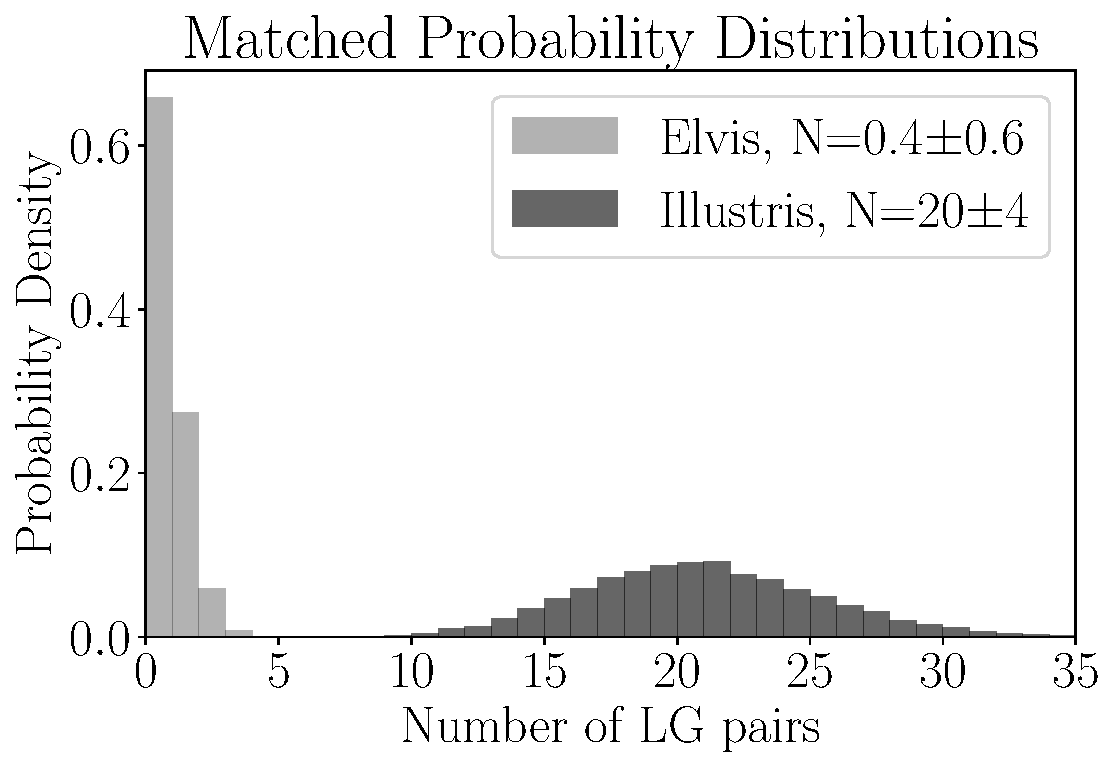
\includegraphics[width=0.47\textwidth]{expected_numbers.pdf}
\caption{Probability distribution for the expected number of pairs
  showing the same degree of atipicality as the Local Group if drawn
  from a sample of 2000 isolated pairs. 
  The distributions correspond to results derived from Illustris-1
  and ELVIS data.
  On average between $0.05\%$ and $0.25\%$ of the isolated pairs should present
  satellite distributions as atypical as the Local Group.
\label{fig:expected_number}}
\end{figure}

\section{Results}
\label{sec:results}


\subsection{Plane Width}

Figure \ref{fig:scatter_width} summarizes the results for the plane
width distributions.
The panel on the left compares the results for the MW and M31
observations against its randomized version. 
The most interesting outcome is that the MW plane width is smaller
than $\approx 98\%$ of the planes computed from the randomized distribution,
while the M31 plane width is consistent with the same distribution. 

\subsection{$c/a$ axis ratio}
Figure \ref{fig:scatter_ca_ratio} shows the results for the minor to
major axis ratio. 
Corresponding in the ELVIS data are in the appendix in Figure
\ref{fig:scatter_elvis}.

The left panel shows the results for the LG compared against its
spherically randomized version.
As expected the $c/a$ ratio in the MW is significantly lower as the
measured values for spherical distributions. 
On the other hand the ratio for M31 is lower than the mean of the
spherical values but still well within its variance.
In contrast to the results for the plane width, this time the
randomized values have symmetrical expectations between the two
galaxies.

The middle panel shows the LG compared against the results from
Illustris. In this case we find a similar trend. The MW is atypical
and M31 is within the variance from the simulation data.
This time, however, there is a single MW-like galaxy out of the total
of 20 that shows an $c/a$ as small as the MW.
The only assymetry evident between the simulated halos is in the
dispersion, the $c/a$ distribution for the massive halos seems to be
wider than it is for the less massive partner. 

The right panel shows the normalized results. 
This highlights the two results mentioned above.
First, the MW shows a low $c/a$ ration close to two standard deviations away
from the mean value of the spherical distribution; this contrasts the
results for M31 which are close to $1$ standard deviation away.
Second, the less massive halos in the Illustris simulation present a
smaller dispersion in their deviations from sphericity than the
its masssive partner.
The MW axis ratio smaller than $\approx 98\%$ of the randomized
satellite distributions.   and its atipicallity is only comparable to
one halo in the Illustris  simulation (none in the ELVIS simulation).


\subsection{$b/a$ axis ratio}

\subsection{Plane alignment}

Figure \ref{fig:scatter_mu} summarizes the Illustris results for the
alignments between the vector normal to the plane and the vector
connecting the two dominant galaxies.
The corresponding results for the ELVIS data are shown in Figure
\ref{fig:scatter_elvis}. 

The first striking impression from the left panel in Figure
\ref{fig:scatter_mu} is that the observations are cornered in
a region of strong alignment, $\mu\approx 1$, for both galaxies. 
In other words, the planes are almost perpendicular to the direction
connecting the two galaxies. 
The result for the spherical randomization corresponds to a uniform
distribution $0\leq \mu\leq 1$ as shown in the same panel.

The middle panel tells a similar story for the results from
Illustris. That is, there isn't a prefered alignment direction from
the simulation. This also holds for ELVIS data.
We quantify this visual impresion by performing a K-S test where the
null hypothesis corresponds to an uniform distribution. 
The results from the K-S test do not allow us to discard the null
hypotesis. 

This information allows us to properly understand the results on the
right panel in Figure \ref{fig:scatter_mu}.
That panel shows the results for the normalized values to the mean and
standard deviation computed from spherically randomized
ditributions.
In this case the LG $\mu$ value has the same probability as any other value
(because it is consistent with an uniform distribution) and the apparent
large distance from the Illustris data must not be interpreted as an
the LG having an atypical alignment. 

We defer to the Section \ref{sec:discussion} our discussion on how
this can be reconciled with other studies that show preferential
infall satellite directions in LCDM simulations.


\begin{table*}
  \centering
  \renewcommand{\arraystretch}{1.2}
  \begin{tabular}{|p{2.5cm}|c|c|c|c|c|c|c|c|}
    \hline
    \multirow{2}{4.0cm}{} & \multicolumn{2}{c|}{\textbf{Observations}} & \multicolumn{2}{c|}{\textbf{Randomized Obs.}} & \multicolumn{2}{c|}{\textbf{Illustris-1}} & \multicolumn{2}{c|}{\textbf{ELVIS}}\\
    % \hline
    % \textbf{Inactive Modes} & \textbf{Description}\\
    \cline{2-9}
    & \textbf{M31} & \textbf{MW} & \textbf{M31} & \textbf{MW} & \textbf{M31} & \textbf{MW}& \textbf{M31} & \textbf{MW}\\
    %\hhline{~--}
    \hline
    Plane width (kpc) & $59\pm 3$  & $22\pm 2$  & $64\pm 12$   & $45\pm 8$     & $70\pm 4$ & $67\pm 2$ & $70\pm 2$& $68\pm 4$ \\\hline
    $c/a$ ratio & $0.45\pm 0.04$ & $0.28\pm 0.03$ & $0.55\pm0.10$ & $0.53\pm 0.10$ & $0.52\pm 0.01$ & $0.53\pm 0.01$ & $0.54\pm 0.01$& $0.49\pm 0.02$ \\ \hline
    $b/a$ ratio & $0.82\pm 0.06$ & $0.78\pm 0.02$ & $0.82\pm0.07$ & $0.81\pm 0.08$ & $0.80\pm 0.01$ & $0.80\pm 0.02$ & $0.80\pm0.01$& $0.81\pm 0.01$\\ \hline
  \end{tabular}
  \caption{Mode Transition Times}
\end{table*}

\section{Discussion}
\subsection{Outlier characterization with a Multivariate Gaussian Model}


Prospects for observational measurement: DESI.

\bibliographystyle{mnras}
\bibliography{Dwarfs}

%% Alignments between galaxies, satellite systems and haloes
%% https://arxiv.org/pdf/1605.01728.pdf

%M31 mass
%% https://arxiv.org/abs/1410.0017

%MW mass
%https://arxiv.org/abs/1407.1078
\newpage
\appendix

\section{Physical Characteristics of the Isolated Pairs samples}

\section{Results from ELVIS}
\begin{figure*}
\centering
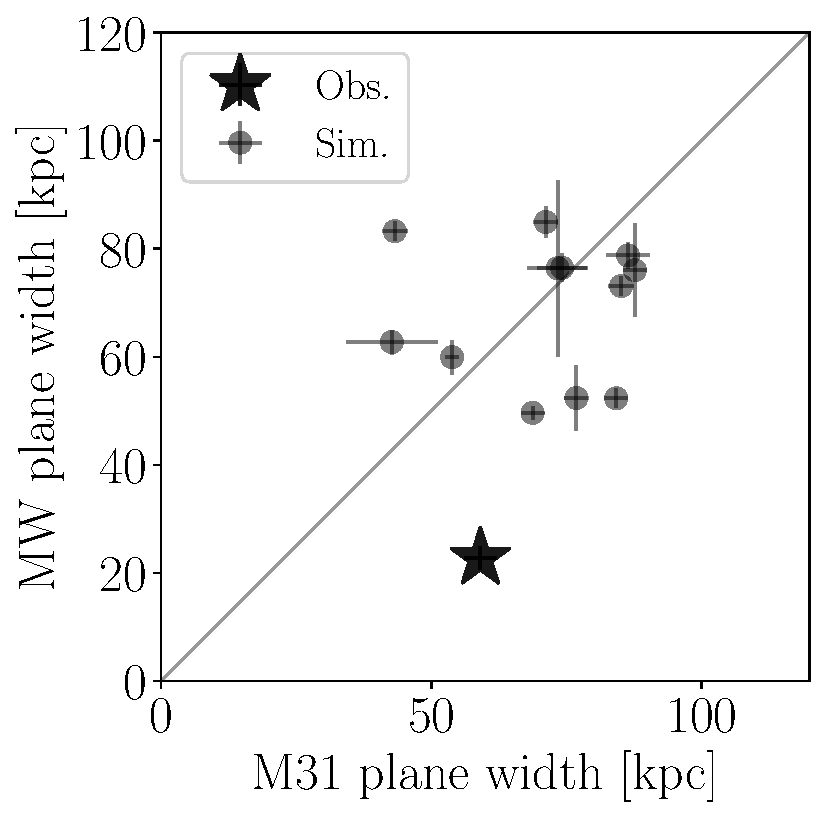
\includegraphics[width=0.24\textwidth]{scatter_ranked_elvis_width.pdf}
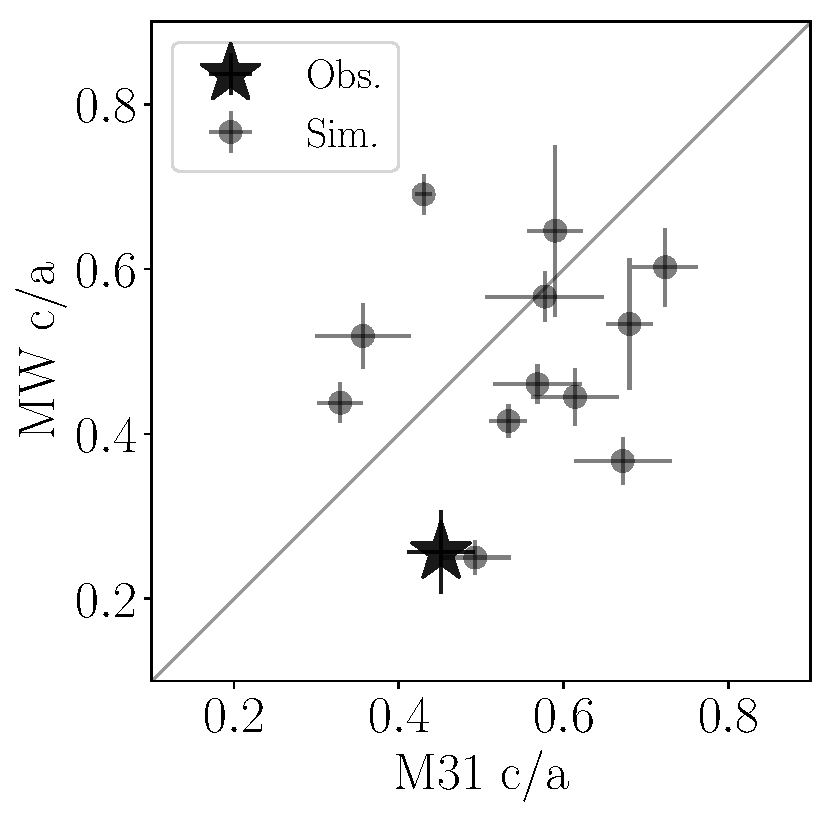
\includegraphics[width=0.24\textwidth]{scatter_ranked_elvis_ca_ratio.pdf}
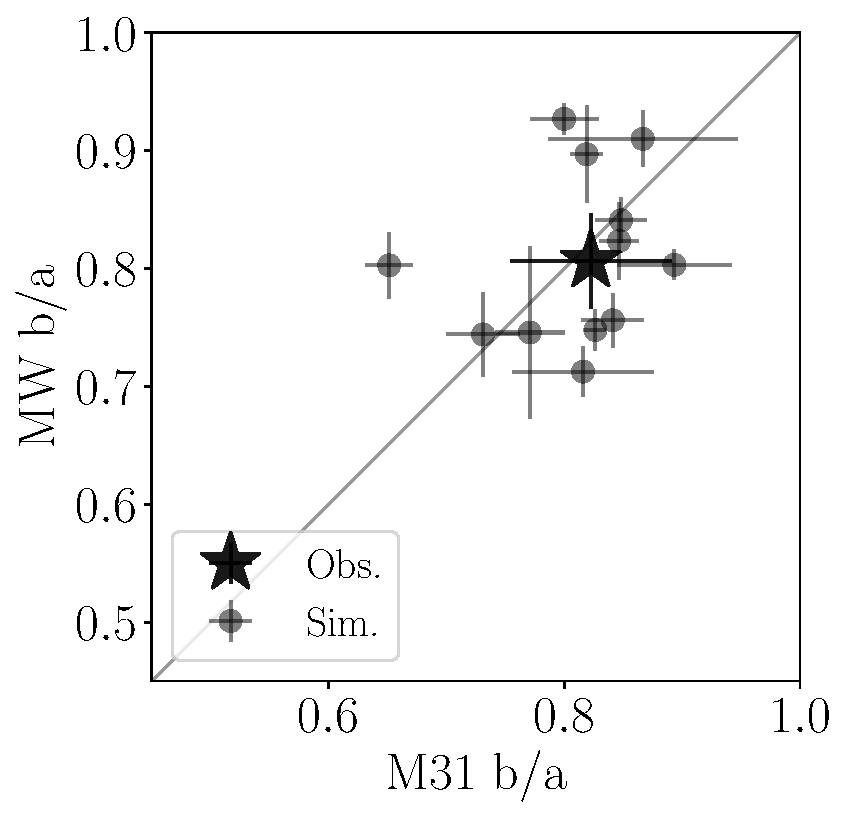
\includegraphics[width=0.24\textwidth]{scatter_ranked_elvis_ba_ratio.pdf}
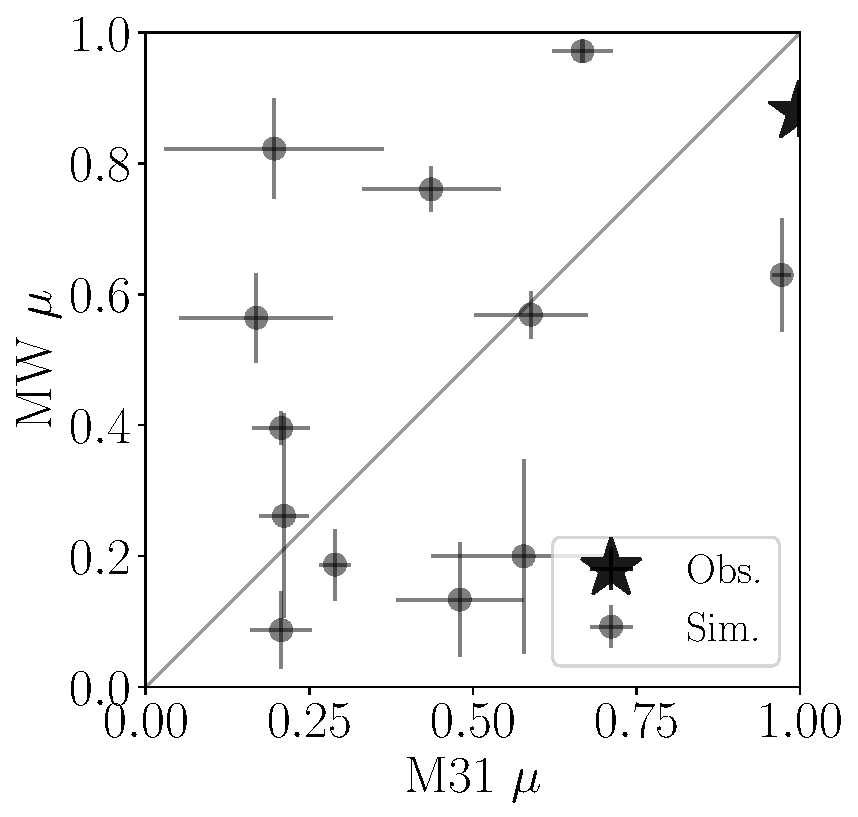
\includegraphics[width=0.24\textwidth]{scatter_ranked_elvis_mu.pdf}
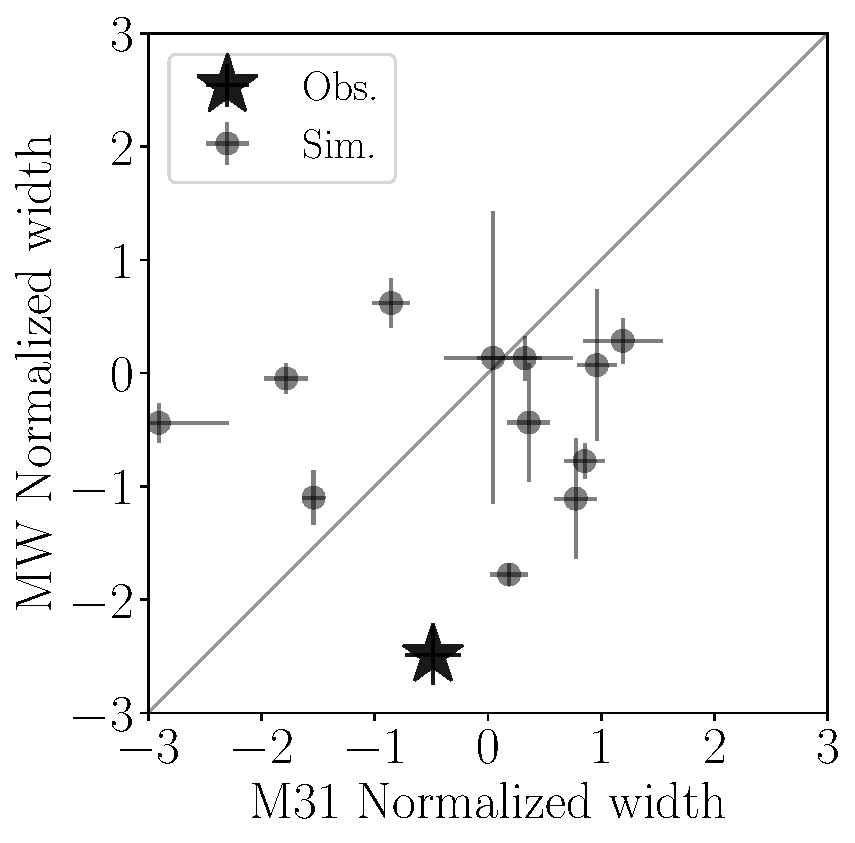
\includegraphics[width=0.24\textwidth]{scatter_norm_ranked_elvis_width.pdf}
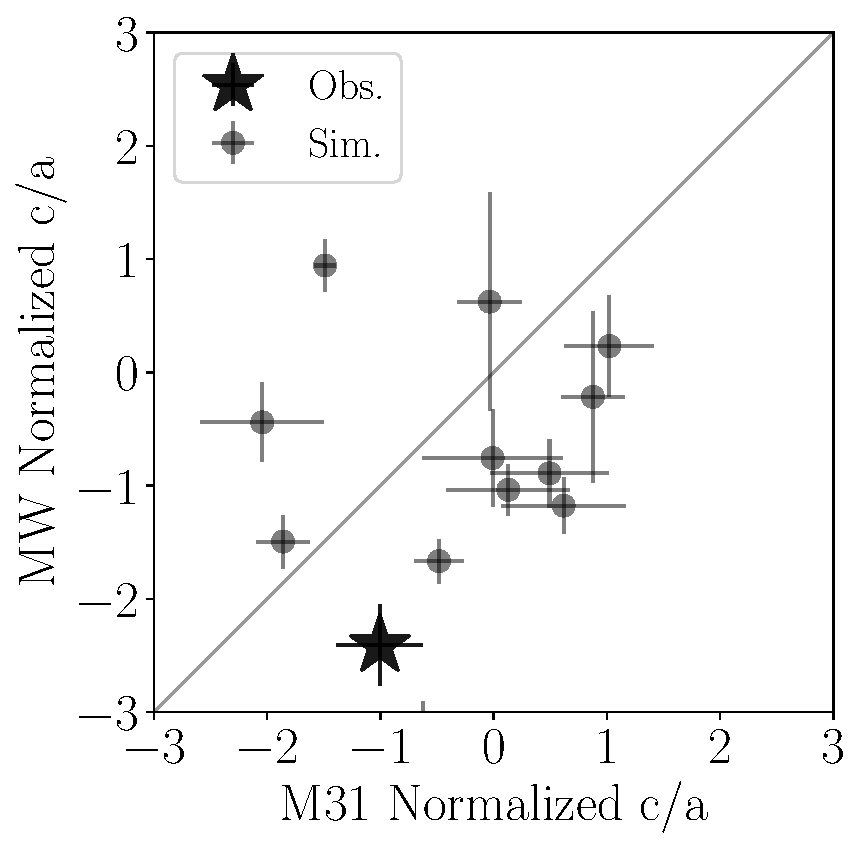
\includegraphics[width=0.24\textwidth]{scatter_norm_ranked_elvis_ca_ratio.pdf}
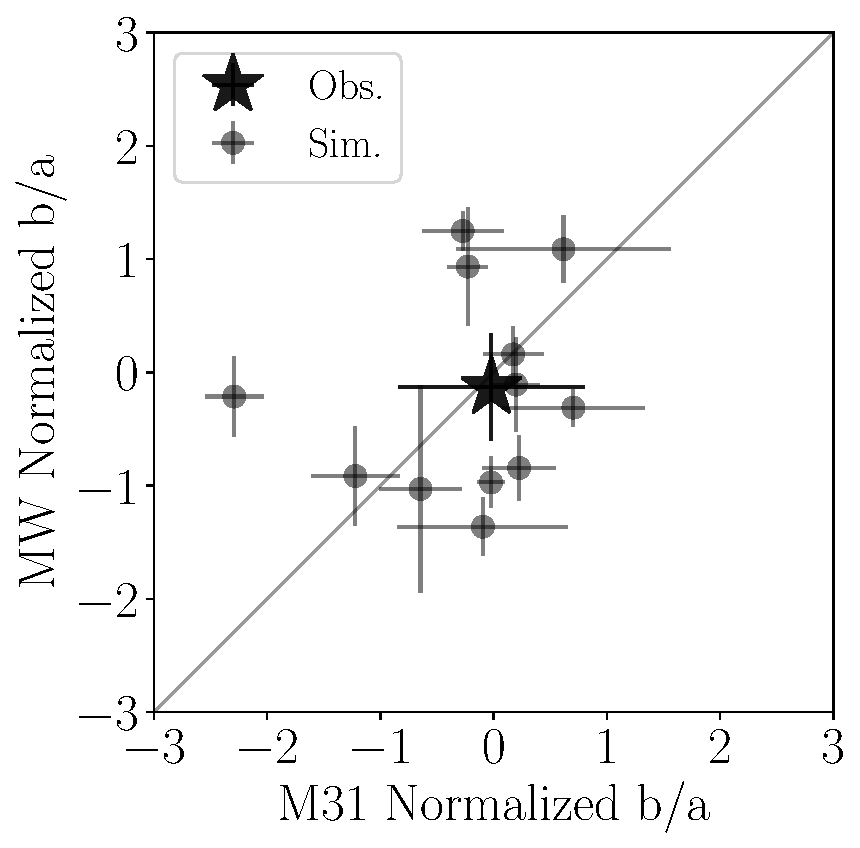
\includegraphics[width=0.24\textwidth]{scatter_norm_ranked_elvis_ba_ratio.pdf}
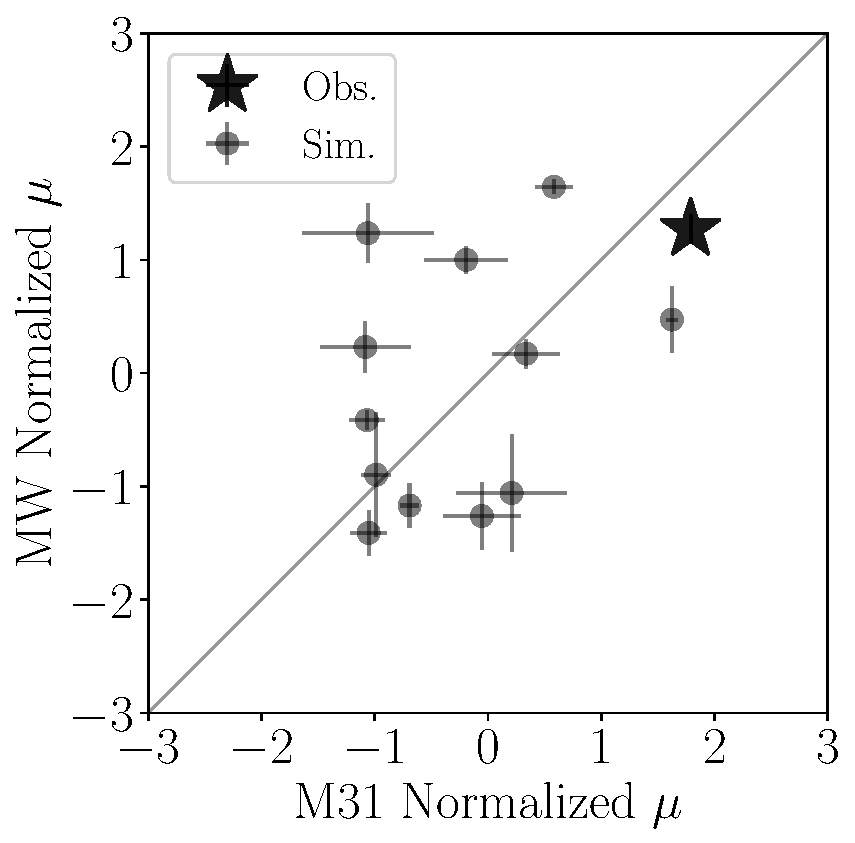
\includegraphics[width=0.24\textwidth]{scatter_norm_ranked_elvis_mu.pdf}
\caption{ELVIs results for the quantities presented for the Illustris-1
  simulation in Figures  \ref{fig:scatter_width},
  \ref{fig:scatter_ca_ratio}, \ref{fig:scatter_ba_ratio} and
  \ref{fig:scatter_mu}.
Upper row corresponds to the raw values from observations and
simulated pairs, while the second row normalizes the same values to
the mean and standard deviation on its spherically randomized
counterparts. 
\label{fig:scatter_elvis}}
\end{figure*}

\begin{figure*}
\centering
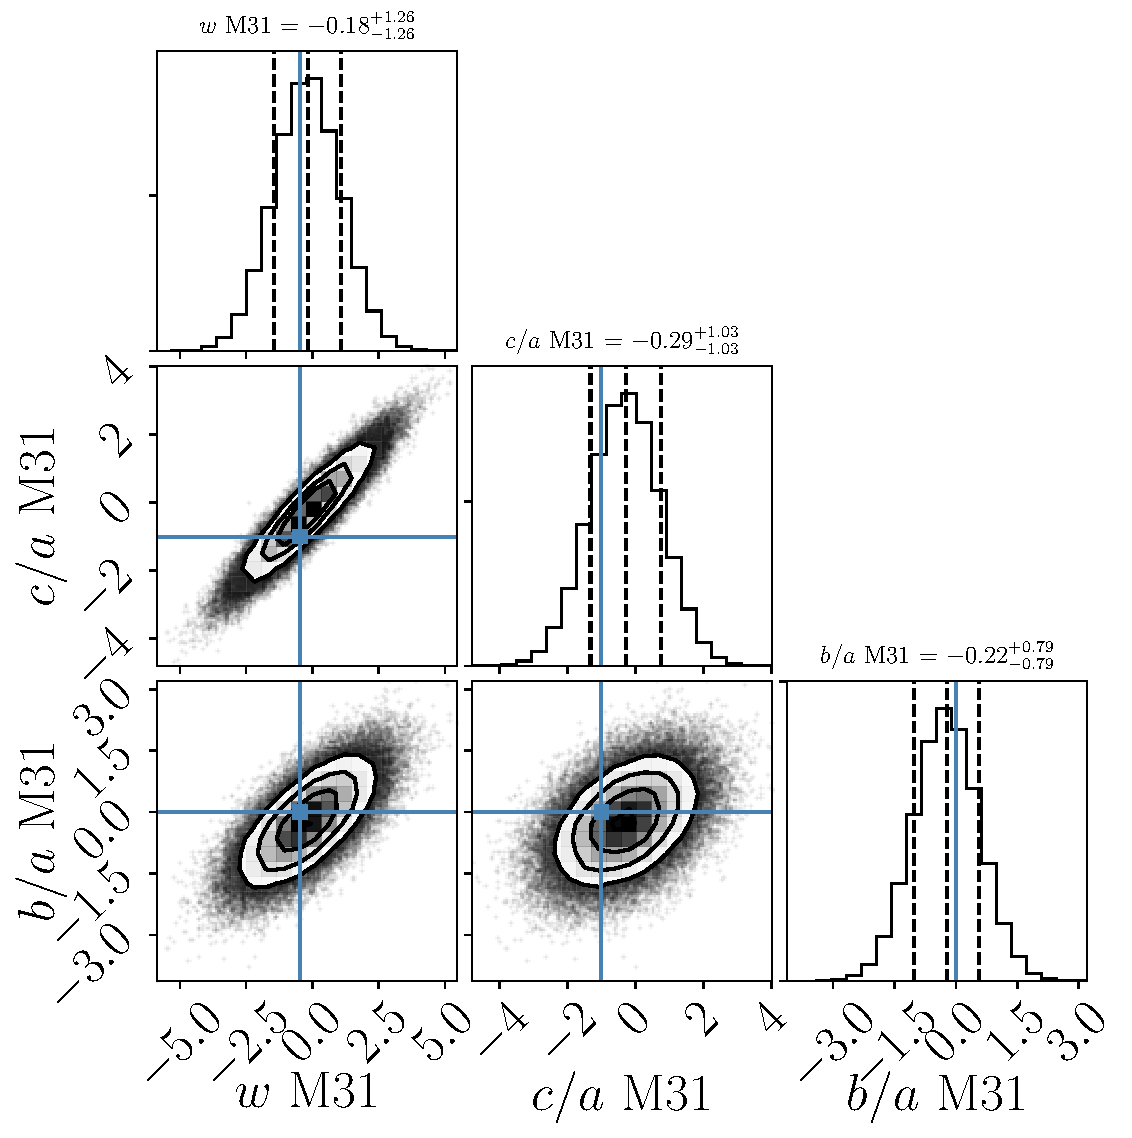
\includegraphics[width=0.45\textwidth]{gaussian_model_elvis_M31.pdf}
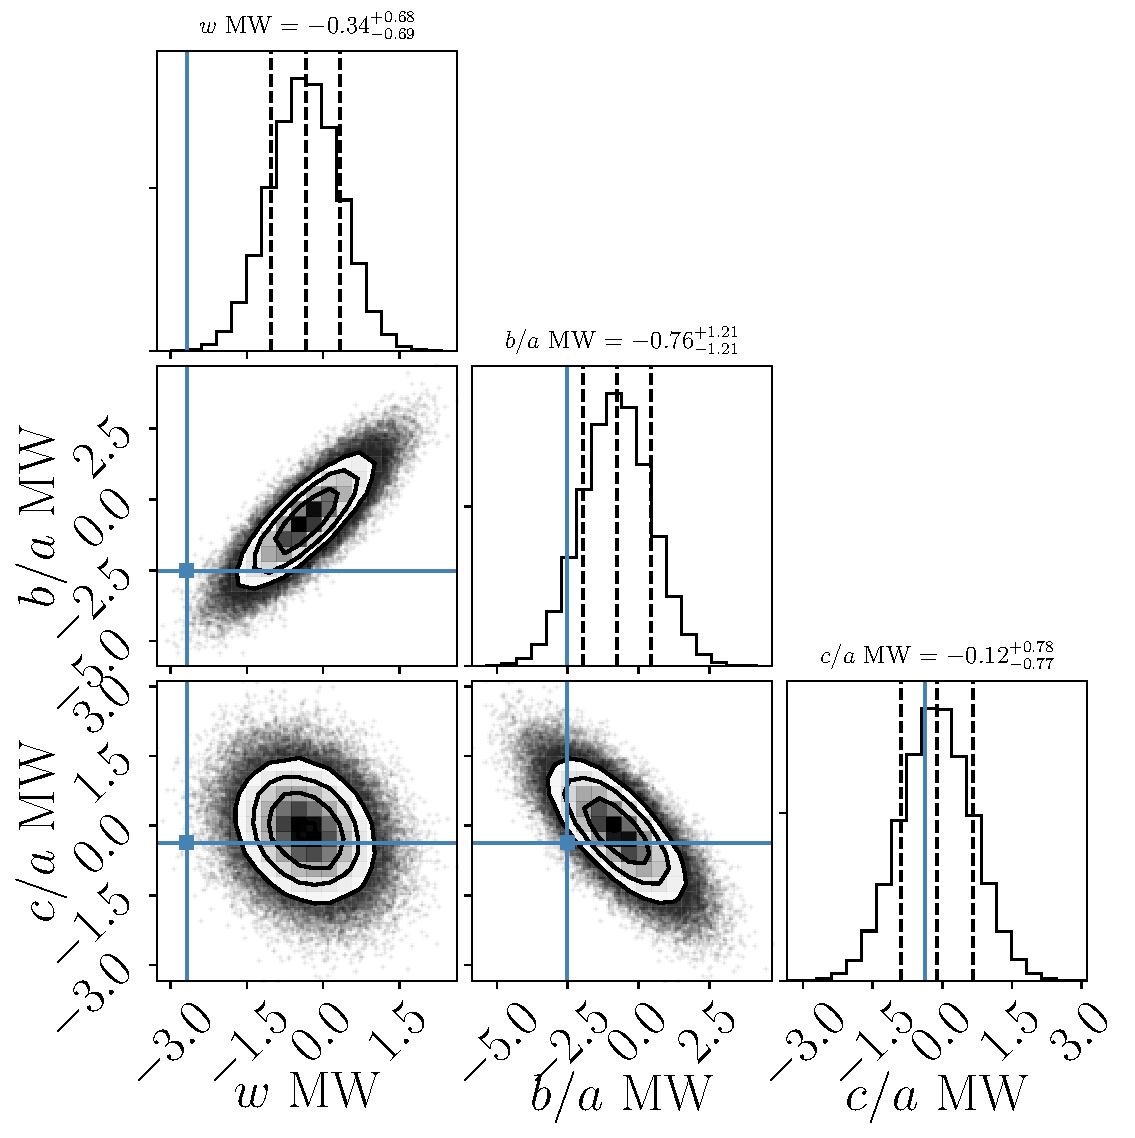
\includegraphics[width=0.45\textwidth]{gaussian_model_elvis_MW.pdf}
\caption{
Same layout as Figure \ref{fig:correlations_illustris}, this time
computed from the ELVIS data.
\label{fig:correlations_elvis}}
\end{figure*}


\end{document}

